\section{Технологический раздел}

\subsection{Выбор языка и библиотеки для разработки средства сбора данных}

В качестве средства реализации была выбрана библиотека Telebot, так как:

\begin{enumerate}
	\item[1.] Функционал приложения не предусматривает сложных операций, в силу чего низкая производительность ЯП Python не скажется на скорости отклика системы;
	\item[2.] ЯП Python позволит в короткий срок реализовать и отладить программный продукт;
	\item[3.] ЯП Python позволит быстро разворачивать приложение на разнообразных операционных системах, поддерживающих интерпретатор Python;
	\item[4.] Telebot предоставляет более тонкую настройку и контроль над запросами и ответами API Telegram.
\end{enumerate}

\subsection{Интерфейс средства сбора данных}

На рисунках \ref{img:teleg1}-\ref{img:teleg4} представлен интерфейс реализованного Telegram-бота.

\begin{figure}[H]
	\centering
	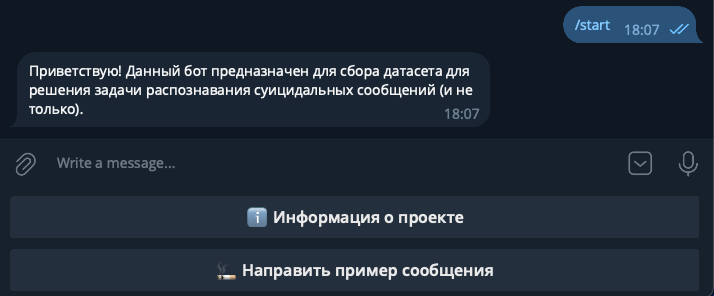
\includegraphics[width=\textwidth]{inc/teleg1.png}
	\caption{ Приветственное сообщение новому пользователю. }
	\label{img:teleg1}
\end{figure}

\begin{figure}[H]
	\centering
	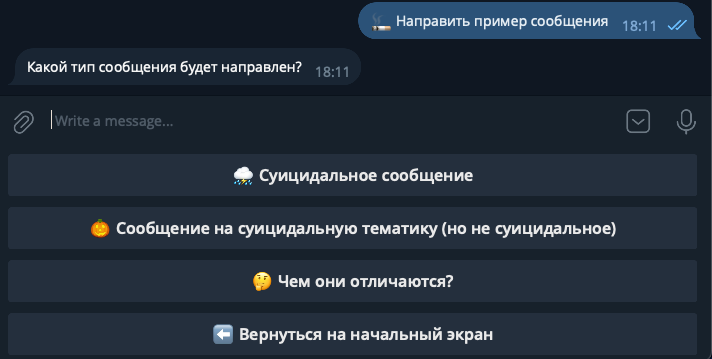
\includegraphics[width=\textwidth]{inc/teleg2.png}
	\caption{ Функционал направления в систему сообщения пользователем. }
	\label{img:teleg2}
\end{figure}

\begin{figure}[H]
	\centering
	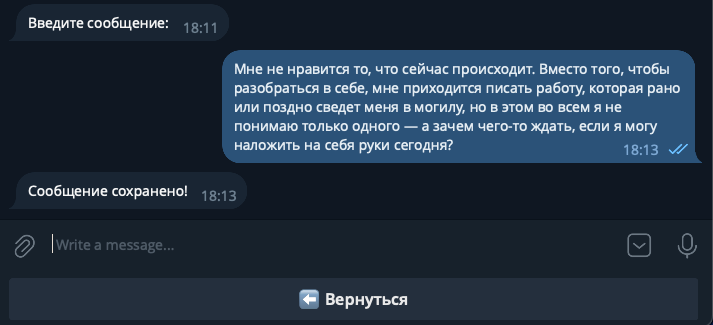
\includegraphics[width=\textwidth]{inc/teleg3.png}
	\caption{ Пример результата направленного в систему суицидального сообщения. }
	\label{img:teleg3}
\end{figure}

\begin{figure}[H]
	\centering
	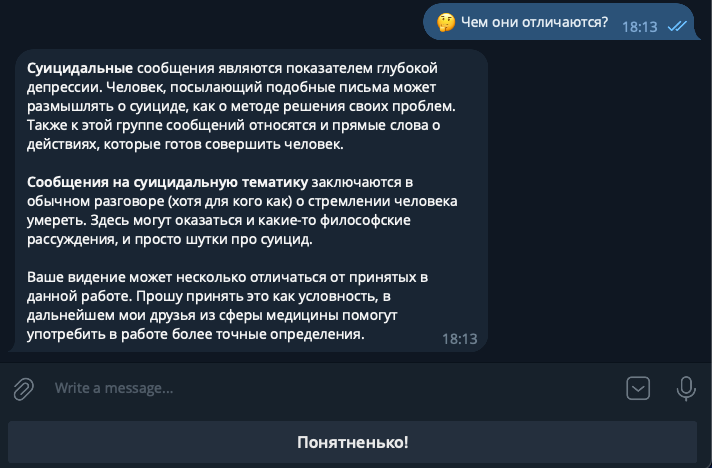
\includegraphics[width=\textwidth]{inc/teleg4.png}
	\caption{ Описание отличий суицидального сообщения и сообщения на суицидальную тематику. }
	\label{img:teleg4}
\end{figure}

\subsection*{Вывод}

В качестве средства реализации была выбрана библиотека Telebot. Продемонстрирован функционал реализованного бота в мессенджере Telegram.